% Options for packages loaded elsewhere
\PassOptionsToPackage{unicode}{hyperref}
\PassOptionsToPackage{hyphens}{url}
%
\documentclass[
]{book}
\usepackage{amsmath,amssymb}
\usepackage{lmodern}
\usepackage{ifxetex,ifluatex}
\ifnum 0\ifxetex 1\fi\ifluatex 1\fi=0 % if pdftex
  \usepackage[T1]{fontenc}
  \usepackage[utf8]{inputenc}
  \usepackage{textcomp} % provide euro and other symbols
\else % if luatex or xetex
  \usepackage{unicode-math}
  \defaultfontfeatures{Scale=MatchLowercase}
  \defaultfontfeatures[\rmfamily]{Ligatures=TeX,Scale=1}
\fi
% Use upquote if available, for straight quotes in verbatim environments
\IfFileExists{upquote.sty}{\usepackage{upquote}}{}
\IfFileExists{microtype.sty}{% use microtype if available
  \usepackage[]{microtype}
  \UseMicrotypeSet[protrusion]{basicmath} % disable protrusion for tt fonts
}{}
\makeatletter
\@ifundefined{KOMAClassName}{% if non-KOMA class
  \IfFileExists{parskip.sty}{%
    \usepackage{parskip}
  }{% else
    \setlength{\parindent}{0pt}
    \setlength{\parskip}{6pt plus 2pt minus 1pt}}
}{% if KOMA class
  \KOMAoptions{parskip=half}}
\makeatother
\usepackage{xcolor}
\IfFileExists{xurl.sty}{\usepackage{xurl}}{} % add URL line breaks if available
\IfFileExists{bookmark.sty}{\usepackage{bookmark}}{\usepackage{hyperref}}
\hypersetup{
  pdftitle={Boosting methods},
  pdfauthor={Emanuel Sommer},
  hidelinks,
  pdfcreator={LaTeX via pandoc}}
\urlstyle{same} % disable monospaced font for URLs
\usepackage{color}
\usepackage{fancyvrb}
\newcommand{\VerbBar}{|}
\newcommand{\VERB}{\Verb[commandchars=\\\{\}]}
\DefineVerbatimEnvironment{Highlighting}{Verbatim}{commandchars=\\\{\}}
% Add ',fontsize=\small' for more characters per line
\usepackage{framed}
\definecolor{shadecolor}{RGB}{248,248,248}
\newenvironment{Shaded}{\begin{snugshade}}{\end{snugshade}}
\newcommand{\AlertTok}[1]{\textcolor[rgb]{0.94,0.16,0.16}{#1}}
\newcommand{\AnnotationTok}[1]{\textcolor[rgb]{0.56,0.35,0.01}{\textbf{\textit{#1}}}}
\newcommand{\AttributeTok}[1]{\textcolor[rgb]{0.77,0.63,0.00}{#1}}
\newcommand{\BaseNTok}[1]{\textcolor[rgb]{0.00,0.00,0.81}{#1}}
\newcommand{\BuiltInTok}[1]{#1}
\newcommand{\CharTok}[1]{\textcolor[rgb]{0.31,0.60,0.02}{#1}}
\newcommand{\CommentTok}[1]{\textcolor[rgb]{0.56,0.35,0.01}{\textit{#1}}}
\newcommand{\CommentVarTok}[1]{\textcolor[rgb]{0.56,0.35,0.01}{\textbf{\textit{#1}}}}
\newcommand{\ConstantTok}[1]{\textcolor[rgb]{0.00,0.00,0.00}{#1}}
\newcommand{\ControlFlowTok}[1]{\textcolor[rgb]{0.13,0.29,0.53}{\textbf{#1}}}
\newcommand{\DataTypeTok}[1]{\textcolor[rgb]{0.13,0.29,0.53}{#1}}
\newcommand{\DecValTok}[1]{\textcolor[rgb]{0.00,0.00,0.81}{#1}}
\newcommand{\DocumentationTok}[1]{\textcolor[rgb]{0.56,0.35,0.01}{\textbf{\textit{#1}}}}
\newcommand{\ErrorTok}[1]{\textcolor[rgb]{0.64,0.00,0.00}{\textbf{#1}}}
\newcommand{\ExtensionTok}[1]{#1}
\newcommand{\FloatTok}[1]{\textcolor[rgb]{0.00,0.00,0.81}{#1}}
\newcommand{\FunctionTok}[1]{\textcolor[rgb]{0.00,0.00,0.00}{#1}}
\newcommand{\ImportTok}[1]{#1}
\newcommand{\InformationTok}[1]{\textcolor[rgb]{0.56,0.35,0.01}{\textbf{\textit{#1}}}}
\newcommand{\KeywordTok}[1]{\textcolor[rgb]{0.13,0.29,0.53}{\textbf{#1}}}
\newcommand{\NormalTok}[1]{#1}
\newcommand{\OperatorTok}[1]{\textcolor[rgb]{0.81,0.36,0.00}{\textbf{#1}}}
\newcommand{\OtherTok}[1]{\textcolor[rgb]{0.56,0.35,0.01}{#1}}
\newcommand{\PreprocessorTok}[1]{\textcolor[rgb]{0.56,0.35,0.01}{\textit{#1}}}
\newcommand{\RegionMarkerTok}[1]{#1}
\newcommand{\SpecialCharTok}[1]{\textcolor[rgb]{0.00,0.00,0.00}{#1}}
\newcommand{\SpecialStringTok}[1]{\textcolor[rgb]{0.31,0.60,0.02}{#1}}
\newcommand{\StringTok}[1]{\textcolor[rgb]{0.31,0.60,0.02}{#1}}
\newcommand{\VariableTok}[1]{\textcolor[rgb]{0.00,0.00,0.00}{#1}}
\newcommand{\VerbatimStringTok}[1]{\textcolor[rgb]{0.31,0.60,0.02}{#1}}
\newcommand{\WarningTok}[1]{\textcolor[rgb]{0.56,0.35,0.01}{\textbf{\textit{#1}}}}
\usepackage{longtable,booktabs,array}
\usepackage{calc} % for calculating minipage widths
% Correct order of tables after \paragraph or \subparagraph
\usepackage{etoolbox}
\makeatletter
\patchcmd\longtable{\par}{\if@noskipsec\mbox{}\fi\par}{}{}
\makeatother
% Allow footnotes in longtable head/foot
\IfFileExists{footnotehyper.sty}{\usepackage{footnotehyper}}{\usepackage{footnote}}
\makesavenoteenv{longtable}
\usepackage{graphicx}
\makeatletter
\def\maxwidth{\ifdim\Gin@nat@width>\linewidth\linewidth\else\Gin@nat@width\fi}
\def\maxheight{\ifdim\Gin@nat@height>\textheight\textheight\else\Gin@nat@height\fi}
\makeatother
% Scale images if necessary, so that they will not overflow the page
% margins by default, and it is still possible to overwrite the defaults
% using explicit options in \includegraphics[width, height, ...]{}
\setkeys{Gin}{width=\maxwidth,height=\maxheight,keepaspectratio}
% Set default figure placement to htbp
\makeatletter
\def\fps@figure{htbp}
\makeatother
\setlength{\emergencystretch}{3em} % prevent overfull lines
\providecommand{\tightlist}{%
  \setlength{\itemsep}{0pt}\setlength{\parskip}{0pt}}
\setcounter{secnumdepth}{5}
\usepackage{booktabs}
\ifluatex
  \usepackage{selnolig}  % disable illegal ligatures
\fi
\usepackage[]{natbib}
\bibliographystyle{apalike}
\newlength{\cslhangindent}
\setlength{\cslhangindent}{1.5em}
\newlength{\csllabelwidth}
\setlength{\csllabelwidth}{3em}
\newenvironment{CSLReferences}[2] % #1 hanging-ident, #2 entry spacing
 {% don't indent paragraphs
  \setlength{\parindent}{0pt}
  % turn on hanging indent if param 1 is 1
  \ifodd #1 \everypar{\setlength{\hangindent}{\cslhangindent}}\ignorespaces\fi
  % set entry spacing
  \ifnum #2 > 0
  \setlength{\parskip}{#2\baselineskip}
  \fi
 }%
 {}
\usepackage{calc}
\newcommand{\CSLBlock}[1]{#1\hfill\break}
\newcommand{\CSLLeftMargin}[1]{\parbox[t]{\csllabelwidth}{#1}}
\newcommand{\CSLRightInline}[1]{\parbox[t]{\linewidth - \csllabelwidth}{#1}\break}
\newcommand{\CSLIndent}[1]{\hspace{\cslhangindent}#1}

\title{Boosting methods}
\author{Emanuel Sommer}
\date{2021-04-07}

\begin{document}
\maketitle

{
\setcounter{tocdepth}{1}
\tableofcontents
}
\hypertarget{prerequisites}{%
\chapter{Prerequisites}\label{prerequisites}}

Here some Notation/ Prerequisites

List:
- CART
- General Machine learining set up (test train split/CV)

\hypertarget{intro}{%
\chapter{Introduction}\label{intro}}

Introduction to the whole setting (seminar topic/ intro to topic maybe mention kaggle wins)

\begin{quote}
``Boosting is one of the most powerful learning ideas introduced in the last
twenty years.'' \citep{elements}
\end{quote}

\hypertarget{theory}{%
\chapter{Theory}\label{theory}}

\hypertarget{the-powerful-idea-of-gradient-boosting}{%
\section{The powerful idea of gradient boosting}\label{the-powerful-idea-of-gradient-boosting}}

As roughly mentioned in the introduction section \ref{intro} the main idea of boosting is to sequentially build `weak' learners that form a powerful ensemble model. It is not totally clear from which field these methods emerged but some claim that the work of Freund and Schapire with respect to PAC learning in the 1990s were instrumental for their growth. \citep{elements} PAC learning can be considered one field within the field of the broader learning theory that tries to find generalization bounds for algorithms that are probably approximately correct (PAC). \citep{pacbounds}

\hypertarget{forward-stagewise-additive-modeling}{%
\subsection{Forward Stagewise Additive Modeling}\label{forward-stagewise-additive-modeling}}

In the setting of the dataset \(\mathcal{D} = \{(y_i,x_i)\ | i \in [N]\}\) with \(x_i \in \mathbb{R}^m\) and \(y_i \in \mathbb{R}\) boosting is fitting the following additive, still quite general, model.

\begin{equation}
  \hat{y_i} = \phi(x_i) = \sum_{k=1}^{K} f_k(x_i), \quad f_k \in \mathcal{F}
  \label{eq:additiveModel}
\end{equation}

Where \(\mathcal{F}\) is the space of learning algorithms that will be narrowed down later on. Additive expansions like this are at the core of many other powerful machine learning algorithms like Neural Networks or Wavelets. \citep{elements}

This leads to the algorithm of Forward Stagewise Additive Modeling. \citep{elements} tbdtbdtbd

\hypertarget{robust-loss-functions-for-regression}{%
\subsection{Robust loss functions for regression}\label{robust-loss-functions-for-regression}}

\hypertarget{off-shelf-performance}{%
\subsection{Off shelf performance}\label{off-shelf-performance}}

Although arguably one of the most famous algorithms in boosting is the Adaboost algorithm for classification, here the focus will be on a regression task and thus Adaboost will not be covered.

\hypertarget{general-gradient-tree-boosting}{%
\section{General gradient tree boosting}\label{general-gradient-tree-boosting}}

first some stuff from elements (more general)

\hypertarget{numerical-optimization}{%
\subsection{numerical optimization}\label{numerical-optimization}}

\hypertarget{gradient-tree-boosting-algorithm-from-elements}{%
\subsection{gradient tree boosting algorithm from elements}\label{gradient-tree-boosting-algorithm-from-elements}}

\hypertarget{problem-of-right-sized-trees}{%
\subsection{problem of right sized trees}\label{problem-of-right-sized-trees}}

\hypertarget{regularisation}{%
\subsection{regularisation}\label{regularisation}}

\begin{figure}
\centering
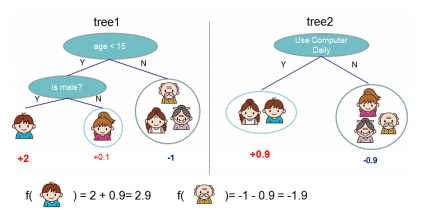
\includegraphics{_pictures/boosting_easy.png}
\caption{Example of an additive tree ensamble\citep{xgboost_paper}}
\end{figure}

\hypertarget{xgboost-a-highly-efficient-implementation}{%
\section{XGBoost a highly efficient implementation}\label{xgboost-a-highly-efficient-implementation}}

use the whole paper

We will cite the great paper!\citep{xgboost_paper}

\hypertarget{eda}{%
\chapter{Expore the data}\label{eda}}

We use the following packages.\citep{tidyverse, tidymodels}

\begin{Shaded}
\begin{Highlighting}[]
\FunctionTok{library}\NormalTok{(tidyverse)}
\FunctionTok{library}\NormalTok{(tidymodels)}
\end{Highlighting}
\end{Shaded}

\hypertarget{train-test-split}{%
\section{Train-test split}\label{train-test-split}}

\begin{Shaded}
\begin{Highlighting}[]
\FunctionTok{set.seed}\NormalTok{(}\DecValTok{2}\NormalTok{)}
\CommentTok{\# ames\_split \textless{}{-} initial\_split(ames, prop = 0.80, strata = Sale\_Price)}
\CommentTok{\# ames\_train \textless{}{-} training(ames\_split)}
\CommentTok{\# ames\_test  \textless{}{-}  testing(ames\_split)}
\end{Highlighting}
\end{Shaded}

\hypertarget{visualize-the-data}{%
\section{Visualize the data}\label{visualize-the-data}}

\begin{itemize}
\item
  pair plots

  \begin{itemize}
  \item
    indiviual main effects
  \item
    correlations
  \end{itemize}
\item
  correlation plot
\item
  individual distributions
\item
  identify categorical features
\item
  feature engineering
\end{itemize}

\hypertarget{create-recipe}{%
\section{Create recipe}\label{create-recipe}}

one for lm (dummify categorical features) and one for the tree based approaches

\begin{Shaded}
\begin{Highlighting}[]
\CommentTok{\# ames\_rec \textless{}{-} }
\CommentTok{\#   recipe(Sale\_Price \textasciitilde{} Neighborhood + Gr\_Liv\_Area + Year\_Built + Bldg\_Type + }
\CommentTok{\#            Latitude + Longitude, data = ames\_train) \%\textgreater{}\%}
\CommentTok{\#   step\_log(Gr\_Liv\_Area, base = 10) \%\textgreater{}\% }
\CommentTok{\#   step\_other(Neighborhood, threshold = 0.01) \%\textgreater{}\% }
\CommentTok{\#   step\_dummy(all\_nominal()) \%\textgreater{}\% }
\CommentTok{\#   step\_interact( \textasciitilde{} Gr\_Liv\_Area:starts\_with("Bldg\_Type\_") ) \%\textgreater{}\% }
\CommentTok{\#   step\_ns(Latitude, Longitude, deg\_free = 20)}
\end{Highlighting}
\end{Shaded}

\hypertarget{modeling}{%
\chapter{Let's boost the models}\label{modeling}}

boooooooooooooooooooooost them (gif here?)

Cite additional model packages.\citep[\citet{ranger_package}]{xgboost_package}

\begin{Shaded}
\begin{Highlighting}[]
\FunctionTok{library}\NormalTok{(xgboost)}
\FunctionTok{library}\NormalTok{(ranger)}
\end{Highlighting}
\end{Shaded}

To do

\begin{enumerate}
\def\labelenumi{\arabic{enumi}.}
\item
  register parallel backend
\item
  create models and workflows
\item
  create resampling objects
\item
  choose tuning method (racing/iterative or grid search)
\item
  tune models and select best ones
\item
  compare final models to test set
\item
  save final model
\end{enumerate}

cite \citep{doParallel_package}

\begin{Shaded}
\begin{Highlighting}[]
\FunctionTok{library}\NormalTok{(doParallel)}

\CommentTok{\# Create a cluster object and then register: }
\NormalTok{cl }\OtherTok{\textless{}{-}} \FunctionTok{makePSOCKcluster}\NormalTok{(}\DecValTok{2}\NormalTok{)}
\FunctionTok{registerDoParallel}\NormalTok{(cl)}

\CommentTok{\# Put at the end:}
\FunctionTok{stopCluster}\NormalTok{(cl)}
\end{Highlighting}
\end{Shaded}

for 2. set engine specific arguments in the set\_engine() function use tune() for parameters that should be tuned (optional tune(``id\_name''))

\begin{Shaded}
\begin{Highlighting}[]
\CommentTok{\# Models:}
\NormalTok{lm\_model }\OtherTok{\textless{}{-}} \FunctionTok{linear\_reg}\NormalTok{() }\SpecialCharTok{\%\textgreater{}\%} 
  \FunctionTok{set\_engine}\NormalTok{(}\StringTok{"lm"}\NormalTok{)}

\NormalTok{rf\_model }\OtherTok{\textless{}{-}} \FunctionTok{rand\_forest}\NormalTok{(}\AttributeTok{trees =} \DecValTok{1000}\NormalTok{) }\SpecialCharTok{\%\textgreater{}\%} 
  \FunctionTok{set\_engine}\NormalTok{(}\StringTok{"ranger"}\NormalTok{) }\SpecialCharTok{\%\textgreater{}\%} 
  \FunctionTok{set\_mode}\NormalTok{(}\StringTok{"regression"}\NormalTok{)}

\NormalTok{boost\_model }\OtherTok{\textless{}{-}} \FunctionTok{boost\_tree}\NormalTok{() }\SpecialCharTok{\%\textgreater{}\%}
  \FunctionTok{set\_engine}\NormalTok{(}\StringTok{"xgboost"}\NormalTok{) }\SpecialCharTok{\%\textgreater{}\%} 
  \FunctionTok{set\_mode}\NormalTok{(}\StringTok{"regression"}\NormalTok{)}
\end{Highlighting}
\end{Shaded}

\begin{Shaded}
\begin{Highlighting}[]
\CommentTok{\# Workflows:}

\CommentTok{\# lm\_wflow \textless{}{-} }
\CommentTok{\#   workflow() \%\textgreater{}\% }
\CommentTok{\#   add\_model(lm\_model) \%\textgreater{}\% }
\CommentTok{\#   add\_recipe()}
\end{Highlighting}
\end{Shaded}

for 3.

\begin{Shaded}
\begin{Highlighting}[]
\CommentTok{\# Create Resampling objects}
\CommentTok{\# set.seed(2)}
\CommentTok{\# ames\_folds \textless{}{-} vfold\_cv(ames\_train, v = 10)}
\end{Highlighting}
\end{Shaded}

for fitting resampling objects without tuning:

\begin{Shaded}
\begin{Highlighting}[]
\CommentTok{\# set.seed(2)}
\CommentTok{\# rf\_res \textless{}{-} rf\_wflow \%\textgreater{}\% }
\CommentTok{\#   fit\_resamples(resamples = ames\_folds)}
\CommentTok{\# \# collect the metrics during resampling with}
\CommentTok{\# collect\_metrics()}
\end{Highlighting}
\end{Shaded}

for 4. and following

\begin{Shaded}
\begin{Highlighting}[]
\CommentTok{\# show the parameters to be tuned with the range}
\CommentTok{\# dials::parameters()}
\CommentTok{\# get and modify the parameters to be tuned with:}
\CommentTok{\# name()}
\CommentTok{\# wflow\_param \%\textgreater{}\% pull\_dials\_object("threshold")}
\CommentTok{\# parameters(ames\_rec) \%\textgreater{}\% }
\CommentTok{\#  update(threshold = threshold(c(0.8, 1.0)))}

\CommentTok{\# finalize for data dependent params}
\CommentTok{\# updated\_param \textless{}{-} }
\CommentTok{\#   workflow() \%\textgreater{}\% }
\CommentTok{\#   add\_model(rf\_spec) \%\textgreater{}\% }
\CommentTok{\#   add\_recipe(pca\_rec) \%\textgreater{}\% }
\CommentTok{\#   parameters() \%\textgreater{}\% }
\CommentTok{\#   finalize(ames\_train)}
\end{Highlighting}
\end{Shaded}

grids: grid\_regular(levels = c(hidden\_units = 3, penalty = 2, epochs = 2)) space filling: grid\_latin\_hypercube(size = 15, original = FALSE) then tune\_grid() function instead of fit\_resamples

\begin{Shaded}
\begin{Highlighting}[]
\NormalTok{roc\_res }\OtherTok{\textless{}{-}} \FunctionTok{metric\_set}\NormalTok{(roc\_auc)}
\FunctionTok{set.seed}\NormalTok{(}\DecValTok{99}\NormalTok{)}
\NormalTok{mlp\_reg\_tune }\OtherTok{\textless{}{-}}
\NormalTok{  mlp\_wflow }\SpecialCharTok{\%\textgreater{}\%}
  \FunctionTok{tune\_grid}\NormalTok{(}
\NormalTok{    cell\_folds,}
    \AttributeTok{grid =}\NormalTok{ mlp\_param }\SpecialCharTok{\%\textgreater{}\%} \FunctionTok{grid\_regular}\NormalTok{(}\AttributeTok{levels =} \DecValTok{3}\NormalTok{),}
    \AttributeTok{metrics =}\NormalTok{ roc\_res}
\NormalTok{  )}

\FunctionTok{autoplot}\NormalTok{(mlp\_reg\_tune) }\SpecialCharTok{+} \FunctionTok{theme}\NormalTok{(}\AttributeTok{legend.position =} \StringTok{"top"}\NormalTok{)}

\FunctionTok{show\_best}\NormalTok{(mlp\_reg\_tune)}

\CommentTok{\# for spacefilling}
\NormalTok{mlp\_sfd\_tune }\OtherTok{\textless{}{-}}
\NormalTok{  mlp\_wflow }\SpecialCharTok{\%\textgreater{}\%}
  \FunctionTok{tune\_grid}\NormalTok{(}
\NormalTok{    cell\_folds,}
    \AttributeTok{grid =} \DecValTok{20}\NormalTok{,}
    \CommentTok{\# Pass in the parameter object to use the appropriate range: }
    \AttributeTok{param\_info =}\NormalTok{ mlp\_param,}
    \AttributeTok{metrics =}\NormalTok{ roc\_res}
\NormalTok{  )}

\FunctionTok{select\_best}\NormalTok{()}
\end{Highlighting}
\end{Shaded}

\begin{Shaded}
\begin{Highlighting}[]
\NormalTok{logistic\_param }\OtherTok{\textless{}{-}} 
  \FunctionTok{tibble}\NormalTok{(}
    \AttributeTok{num\_comp =} \DecValTok{0}\NormalTok{,}
    \AttributeTok{epochs =} \DecValTok{125}\NormalTok{,}
    \AttributeTok{hidden\_units =} \DecValTok{1}\NormalTok{,}
    \AttributeTok{penalty =} \DecValTok{1}
\NormalTok{  )}

\NormalTok{final\_mlp\_wflow }\OtherTok{\textless{}{-}} 
\NormalTok{  mlp\_wflow }\SpecialCharTok{\%\textgreater{}\%} 
  \FunctionTok{finalize\_workflow}\NormalTok{(logistic\_param)}

\NormalTok{final\_mlp\_fit }\OtherTok{\textless{}{-}} 
\NormalTok{  final\_mlp\_wflow }\SpecialCharTok{\%\textgreater{}\%} 
  \FunctionTok{fit}\NormalTok{(cells)}
\end{Highlighting}
\end{Shaded}

Racing:

\begin{Shaded}
\begin{Highlighting}[]
\FunctionTok{library}\NormalTok{(finetune) }\CommentTok{\# if used to be cited}

\FunctionTok{set.seed}\NormalTok{(}\DecValTok{99}\NormalTok{)}
\NormalTok{mlp\_sfd\_race }\OtherTok{\textless{}{-}}
\NormalTok{  mlp\_wflow }\SpecialCharTok{\%\textgreater{}\%}
  \FunctionTok{tune\_race\_anova}\NormalTok{(}
\NormalTok{    cell\_folds,}
    \AttributeTok{grid =} \DecValTok{20}\NormalTok{,}
    \AttributeTok{param\_info =}\NormalTok{ mlp\_param,}
    \AttributeTok{metrics =}\NormalTok{ roc\_res,}
    \AttributeTok{control =} \FunctionTok{control\_race}\NormalTok{(}\AttributeTok{verbose\_elim =} \ConstantTok{TRUE}\NormalTok{)}
\NormalTok{  )}
\end{Highlighting}
\end{Shaded}

Here no iterative search as big parameter space, could be done after grid search or for single parameters. (If then Simulated Annealing)

\hypertarget{conclusion}{%
\chapter{Conclusion}\label{conclusion}}

Let's wrap it up!

\hypertarget{references}{%
\chapter{References}\label{references}}

\hypertarget{refs}{}
\begin{CSLReferences}{0}{0}
\end{CSLReferences}

  \bibliography{book.bib,packages.bib}

\end{document}
